\documentclass{article}
\newcommand{\mydate}{September 18, 2025}
\newcommand{\mytitle}{GP1 HW2}
\title{\textbf{\mytitle}}
\author{Jiete XUE\thanks{SID: 20253121013}}
\date{\mydate}
\usepackage{fancyhdr}
\pagestyle{fancy}
\fancyhf{}
\fancyhead[C]{\mytitle }
\fancyhead[R]{Jiete Xue}
\fancyhead[L]{\mydate}
\fancyfoot[C]{\thepage}
\usepackage{graphicx}
\usepackage{amsthm}
\usepackage{amsmath}
\usepackage{amssymb}
\usepackage{subcaption}
\usepackage{physics}

%% 右矢
%\ket{\psi}          % 输出:|ψ⟩
%\ket{\psi(t)}       % 输出:|ψ(t)⟩
%
%% 左矢
%\bra{\phi}          % 输出:⟨φ|
%
%% 期望值
%\expval{\hat{A}}    % 输出:⟨Â⟩
%\expval{\hat{A}}{\psi}  % 输出:⟨ψ|Â|ψ⟩
%
%% 对易子
%\comm{\hat{A}}{\hat{B}}  % 输出:[Â, B̂]
\newtheoremstyle{1}{}{}{}{}{\bfseries}{}{\newline}{}
\theoremstyle{1}
\newtheorem{problem}{Problem}
\usepackage{chngcntr}
\counterwithin{equation}{problem}
\newcommand{\pa}{\partial}
\newcommand{\rn}[1]{\romannumeral #1\relax}

\begin{document}

\maketitle
\begin{problem}
    We have
    \begin{equation}
        \dot{v}=\frac{1}{2}\frac{\dd(v^2)}{\dd x},
    \end{equation}
    Plug in Newton's second law, we have
    \begin{equation}
        F=m\dot{v}=\frac{1}{2}m\frac{\dd(v^2)}{\dd x}.
    \end{equation}
Then we can do the integration both sides.
\begin{equation}
    v^2=v_0^2+\frac{2}{m}\int_{x_0}^{x}F\,\dd x.
\end{equation}
In particular, if $F$ is a constant, we have
\begin{equation}
    v^2=v_0^2+\frac{2}{m}F(x-x_0).
\end{equation}
\end{problem}
\begin{problem}
(1)
            \begin{eqnarray}
                m\dot{v}_x&=&qv_yB\\
                m\dot{v}_y&=&-qv_xB+qE\\\label{2.2}
                m\dot{v}_z&=&0\label{2.3}
            \end{eqnarray}
    Since $v_{z0}=0$ and by \eqref{2.3}, we have
    \begin{equation}
        v_z(t)=0.
    \end{equation}
    So the motion remains in $z= 0$ plane.
\newline
(2) We need $\dot{v}_y=0$ to satisfy particle moving unreflected through the field. Then, by \eqref{2.2},
\begin{equation}
    v_x=\frac{E}{B}
\end{equation}
\newline
(3) Let $r=x+iy$, where $i$ is the imaginary unit. Rewrite the equation in 1. as:
\begin{equation}
    m\ddot{r}=iq(E-\dot{r}B).
\end{equation}
Then we can deduce that 
\begin{equation}
    r=\frac{i}{2m}qEt^2+Ae^{-iqBt/m}+C.
\end{equation}
By the initial condition,
\begin{equation}
    r(0)=0,\ \dot{r}(0)=v_{x0},
\end{equation}
we have
\begin{equation}
    r(t)=\frac{i}{2m}qEt^2+\frac{iv_{x0}m}{qB}\left( e^{-iqBt/m}-1\right),
\end{equation}
\begin{equation}
    \dot{r}(t)=i\frac{qE}{m}t+v_{x0}\left(e^{-iqBt/m}-1\right).
\end{equation}
(4) Reparameterize $r$ to 
\begin{equation}
    r=i\eta t^2+i\epsilon \left( e^{-i\omega t}-1\right),
\end{equation}
where $\eta$ and $\epsilon$ are both real numbers.
\begin{figure}[htbp]
    \centering
    \begin{subfigure}{0.45\textwidth}
        \centering
        \includegraphics[width=\textwidth]{initial state.png}
        \caption{In the initial stage}
        \label{fig:sub1}
    \end{subfigure}
    \hfill % 添加水平填充,使图片分开
    \begin{subfigure}{0.45\textwidth}
        \centering
        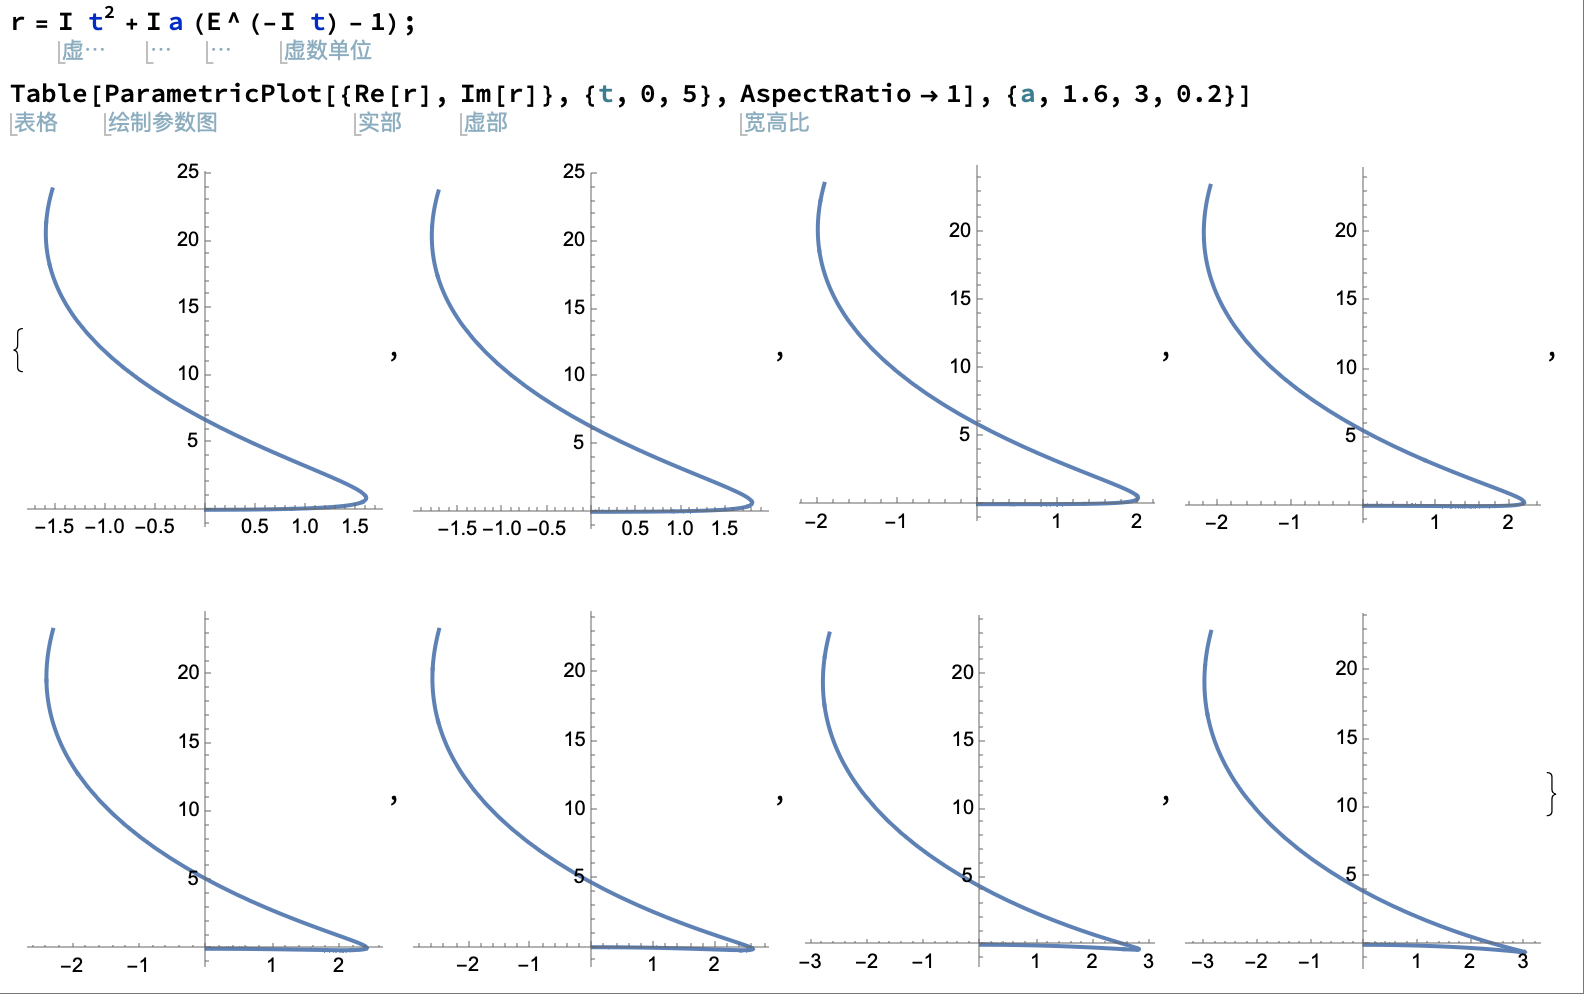
\includegraphics[width=\textwidth]{following.png}
        \caption{In the following stage}
        \label{fig:sub2}
    \end{subfigure}
    \caption{The motion of a charged particle in a electromagnetic field.}
    \label{fig:main}
\end{figure}

\end{problem}
\begin{problem}
    We just need to consider only one direction, and the others will be the same. Assume that 
    \begin{equation}
        v_{\rho0}=v_0\cos\theta,\ v_{z0}=v_0\sin\theta.
    \end{equation}
    Then, 
    \begin{equation}\label{3.2}
        z=-\frac{1}{2}g\left(\frac{\rho}{v_0}\right)^2(1+\tan^2\theta)+\rho \tan\theta.
    \end{equation}
    We want to know the boundary when $\theta$ have taken all the values it can reach.
    \begin{equation}
        \frac{\pa z}{\pa (\tan\theta)}=-g\left(\frac{\rho}{v_0}\right)^2\tan\theta+\rho=0.
    \end{equation}
Plug in \eqref{3.2}, we obtain:
\begin{equation}
    z=\frac{v_0^2}{2g}-\frac{1}{2}g\frac{\rho^2}{v_0^2}.
\end{equation}
That's exactly the boundary.
\end{problem}
\begin{problem}[Fall wtih resistance]
   (1) At this scale and speed, we suppose quadratic drag force take the main role. Set down straight as the positive direction of axis $z$.
   \begin{equation}
    mg-\frac{\kappa \pi}{4}D^2\rho_a \dot{z}^2=m\ddot{z}.
   \end{equation} 
   Let $z=z^{(0)}+z^{(1)},z^{(1)}<<z^{(0)}$,
   \begin{equation}
    z^{(0)}=\frac{1}{2}gt^2.
   \end{equation}
   \begin{equation}
    -\frac{\kappa \pi}{4}D^2\rho_a (\dot{z}^{(0)})^2\approx m\ddot{z}^{(1)}.
   \end{equation}
Thus,
\begin{equation}
    z^{(1)}(t)\approx-\frac{\kappa\pi}{480}\frac{D^2g^2\rho_a}{m}t^6=-\epsilon t^6.
\end{equation}
Let $t=t^{(0)}+t^{(1)},t^{(0)}<<t^{(1)} $,
\begin{equation}
    t^{(0)}=\sqrt{\frac{2z}{g}}\approx3.35s,
\end{equation}
\begin{equation}
    gt^{(0)}t^{(1)}-\epsilon \left(t^{(0)}\right)^6\approx0.
\end{equation}
Hence,
\begin{equation}
    t^{(1)}\approx\frac{\epsilon (t^{(0)})^5}{g}.
\end{equation}
\begin{equation}
    \Delta t\approx\frac{\Delta \epsilon(t^{(0)})^5}{g}\approx0.42s
\end{equation}
It is difficult to tell difference at the top of the tower. But the people at the bottom can find they didn't hit the ground at the same time.
\newline
(2)
I think this problem makes no sense, and I have no reason to believe that the formula you give still holds in such high speed. So I refuse to answer.
\end{problem}
\newpage
\begin{problem}[The Longest Fall]
(1) 
\begin{equation}
    \Delta m_1=\sigma \Delta \Omega r_1^2,\ \Delta m_2=\sigma \Delta \Omega r_2^2.
\end{equation}
\begin{equation}
    F_1=\frac{G\Delta m_1 m}{r_1^2}=\frac{G\Delta m_2 m}{r_2^2}=F_2.
\end{equation}
That means the force generate by the opposite spheres cancel each other.
\newline
(2) Suppose the density of the spheres is $\rho$, then 
\begin{equation}
    F(r)=-\frac{G\rho \left(\frac{4\pi}{3}r^3\right)m}{r^2}=-\frac{4\pi \rho G m}{3}r.
\end{equation}
By Newton's second law, we have
\begin{equation}
    m\ddot{r}=-\frac{4\pi \rho Gm}{3}r.
\end{equation}
Its solution is:
\begin{equation}
    r(t)=R\cos(\omega t+\phi).
\end{equation}
Where $R$ is the amplitude, $\omega=\sqrt{\frac{4\pi \rho G}{3}}$ is the angular frequency and $\phi$ is the phase. It is a harmonic oscillation, and its period is 
\begin{equation}
    T=2\pi\sqrt{\frac{3}{4\pi \rho G}{}}.
\end{equation}
(3) For satellite, 
\begin{equation}
    m\dot{\theta}^2R=\frac{Gm\rho \frac{4\pi}{3}R^3}{R^2}.
\end{equation}
Hence, 
\begin{equation}
    \dot{\theta}=\sqrt{\frac{3}{4\pi \rho G}{}}
\end{equation}
\begin{equation}
    proj=R\cos\theta=R\cos\left(\sqrt{\frac{4\pi \rho G}{3}}t+\phi\right)=r(t).
\end{equation}
(4)
\begin{equation}
    \vec{F}(\vec{r})=-\frac{4\pi\rho  Gm}{3}\vec{r}.
\end{equation}
Let $\vec{\tau}$ be the direction of the tunnel. Then, we have the projection of $\vec{F}$ in the direction of $\vec{\tau}$ and the motion equation:
\begin{equation}
    \vec{F}(\vec{\tau}\cdot\vec{r})=\vec{\tau}\cdot\vec{F}(\vec{r})=\vec{\tau }\cdot\ddot{\vec{r}}=\frac{\dd^2}{\dd t^2}(\vec{\tau}\cdot\vec{r}).
\end{equation}
Thus,
\begin{equation}
    \vec{\tau}\cdot\vec{r}=R\cos\left(\sqrt{\frac{4\pi \rho G}{3}}t+\phi\right).
\end{equation}
It is still a harmonic oscillation with the same period.
\end{problem}
\end{document}